\documentclass[12pt]{article}
\usepackage{sbc-template}
\usepackage[utf8]{inputenc}
\usepackage[T1]{fontenc}
\usepackage{babel}
\babelprovide[main,import=pt-BR]{brazil}
\usepackage{graphicx,url,booktabs,listings,textcomp}
\usepackage{pdflscape}
\sloppy
\renewcommand{\topfraction}{0.9}
\renewcommand{\textfraction}{0.08}
\renewcommand{\floatpagefraction}{0.8}
\lstset{language=SQL,basicstyle=\ttfamily\fontsize{6.5}{7}\selectfont,
  keywordstyle=\bfseries,commentstyle=\itshape,showstringspaces=false,
  columns=fullflexible,keepspaces=true,breaklines=true,breakatwhitespace=true,upquote=true,
  aboveskip=4pt,belowskip=4pt,
  literate={Á}{{\'A}}1 {Ã}{{\~A}}1 {Ç}{{\c C}}1 {É}{{\'E}}1
    {Ó}{{\'O}}1 {Ú}{{\'U}}1 {ã}{{\~a}}1 {ç}{{\c c}}1
    {õ}{{\~o}}1 {í}{{\'i}}1 {á}{{\'a}}1 {é}{{\'e}}1 {ó}{{\'o}}1}

\title{Descrição e preparação dos dados do serviço 156 de Curitiba\\
nos anos de 2017 e 2018}
\author{Enzo Nakamura Kira\inst{1}, Gustavo Henrique Bruno dos Santos\inst{1}}
\address{Universidade Tecnológica Federal do Paraná (UTFPR)\\Curitiba -- PR -- Brasil}

\begin{document}
\maketitle
\begin{abstract}
This paper summarizes the preparation of Curitiba's 156 service data from
2017 and 2018. We used 24 CSV files and Python to handle missing values, remove
duplicates and load the data into Postgiscwb. We describe data quality and the
addition of geographic coordinates. We also assign geocoded social and lighting
requests to neighborhoods. 96.88\% of social requests are within
500 m of a lighting request, versus 30.21\% within 100 m. These service
requests do not allow us to assess violence risk.
\end{abstract}
\begin{resumo}
Este artigo resume a preparação dos dados do serviço 156 de Curitiba nos anos
de 2017 e 2018. Usamos 24 arquivos CSV e Python para tratar valores nulos,
remover duplicatas e inserir os dados no Postgiscwb. Apresentamos a qualidade dos
dados e a inclusão de coordenadas. Também relacionamos pedidos sociais e de
iluminação aos bairros: 96,88\% dos pedidos sociais estão a até 500 m de um
pedido de iluminação; esse percentual cai para 30,21\% quando a distância
considerada é de 100 m. Esses registros não permitem avaliar o risco de violência.
\end{resumo}

\section{Introdução}
Utilizamos dados do serviço 156 de Curitiba referentes a 2017 e 2018, inseridos
na tabela \texttt{bd2\_156\_enzo\_gustavo} do Postgiscwb. Neste artigo, resumimos
a preparação dos registros de solicitações e atendimentos, os problemas
encontrados e a inclusão de coordenadas geográficas. A análise busca responder
à seguinte pergunta: como se distribuem as demandas de abordagem social e
manutenção da iluminação entre os bairros, e qual proporção dos registros sociais
está a até 500 m de uma demanda de iluminação?

\section{Descrição dos dados e inserção}
Usamos 24 arquivos \texttt{.csv}, com cabeçalhos em português. Após a limpeza
em Python e a inserção no banco, a tabela final ficou com 142.221 tuplas.
Valores nulos, sobretudo em datas, foram tratados; verificamos o tamanho máximo
dos textos e removemos espaços no início e no fim dos textos. O processamento levou cerca
de dois minutos e a inserção, três minutos.

Encontramos variações de maiúsculas, minúsculas e acentuação, além de 15.129
tuplas com espaços extras e 927 com caracteres de controle. Nas quatro colunas de texto
livre, foram encontrados padrões de telefone em 4.371 tuplas, e-mail em 162,
CPF em 39 e RG em 11. As buscas por nomes produziram falsos positivos. A
anonimização foi proposta, mas não concluída nessa etapa.

Adicionamos \texttt{geom}, do tipo \texttt{POINT} com SRID 4326, associando
logradouro e número à tabela \texttt{alvara\_enderecos}; criamos um índice
GiST. O comando de atualização retornou 48.709 linhas afetadas, mas 31.605 das 142.221
tuplas tinham geometria não nula. A diferença não foi explicada. Há 79.203
registros de 2016; o recorte de 2017--2018 contém 63.018, dos quais 15.841
(25,14\%) têm coordenadas. Nesse recorte, os valores de \texttt{SOLICITACAO}
são únicos e não nulos, e a última data é 22/11/2018. Cruzamos esses pontos com
\texttt{limites\_legais.divisa\_de\_bairros}: 75 polígonos válidos em EPSG:29192.
Os textos pessoais e pontos individuais não foram exportados.

\section{Análise espacial}
\subsection{Seleção dos dados e metodologia}
Consideramos \texttt{TIPO} igual a \texttt{SOLICITAÇÃO} ou \texttt{RECLAMAÇÃO},
após padronizar maiúsculas e minúsculas e remover espaços externos. A categoria social reúne assuntos
iniciados por \texttt{ABORDAGEM SOCIAL DE RUA}, incluindo adulto e criança.
Para iluminação, usamos \texttt{ILUMINAÇÃO PÚBLICA} e a subdivisão
\texttt{MANUTENÇÃO DE LUMINÁRIAS}; excluímos implantação, taxas, elogios e
recadastros. Pedidos de manutenção indicam demanda por reparo, mas não comprovam
que havia lâmpadas apagadas. Encontramos 2.546 registros sociais e 6.717 de iluminação;
somente 513 (20,15\%) e 1.359 (20,23\%), respectivamente, possuem coordenadas.

Transformamos pontos de EPSG:4326 e bairros de EPSG:29192 (SAD69 / UTM 22S)
para EPSG:31982 (SIRGAS 2000 / UTM 22S), sem alterar as tabelas originais.
A consulta usa quatro funções espaciais \cite{postgis}: \texttt{ST\_Transform}
compatibiliza os sistemas; \texttt{ST\_Covers} associa pontos ao interior ou
limite de cada bairro; \texttt{ST\_Area} calcula áreas; e \texttt{ST\_DWithin}
testa distâncias euclidianas em metros. Não são distâncias de caminhada.
Todos os pontos selecionados são válidos e pertencem a exatamente um bairro.

Para cada bairro $b$, calculamos contagens sociais $S_b$ e de iluminação $L_b$,
densidades $S_b/A_b$ e $L_b/A_b$, com $A_b$ em km$^2$, e
\(P_b(r)=100\,N_b(r)/S_b\), em que $N_b(r)$ conta registros sociais com pelo
menos um pedido de iluminação a até $r$ metros. A busca inclui iluminação de
bairros vizinhos; \texttt{EXISTS} evita contar o mesmo pedido social várias
vezes. Quando $S_b=0$, o percentual não é calculado. Além do raio de 500 m,
avaliamos 100 e 250 m para verificar como o resultado varia com o raio.

\subsection{Resultados e visualização}
Há registros sociais georreferenciados em 57 dos 75 bairros. O Centro concentra
158 deles (30,80\%) e 187 demandas de iluminação; os cinco bairros da
Tabela~\ref{tab:ranking} reúnem 50,49\% dos registros sociais. A Cidade
Industrial de Curitiba tem a segunda maior contagem de iluminação (87), seguida
do Sítio Cercado (57). O Centro também apresenta as maiores densidades:
48,13 registros sociais e 56,96 de iluminação por km$^2$.

\begin{table}[htbp]
\centering
\caption{Cinco bairros com mais registros sociais georreferenciados.
$D_S$ e $D_L$: registros/km$^2$; $P_b(500)$: percentual de proximidade.}
\label{tab:ranking}
\small
\begin{tabular}{lrrrrr}
\toprule
Bairro & $S_b$ & $L_b$ & $D_S$ & $D_L$ & $P_b(500)$ (\%) \\
\midrule
Centro & 158 & 187 & 48,13 & 56,96 & 100,00 \\
Rebouças & 31 & 22 & 10,45 & 7,42 & 100,00 \\
Água Verde & 27 & 54 & 5,66 & 11,31 & 100,00 \\
Batel & 25 & 15 & 14,39 & 8,63 & 100,00 \\
Jardim Botânico & 18 & 5 & 6,53 & 1,81 & 100,00 \\
\bottomrule
\end{tabular}
\end{table}

No conjunto da cidade, 497 dos 513 registros sociais (96,88\%) estão a até
500 m de uma demanda de iluminação. A até 250 m, são 379 registros (73,88\%);
a até 100 m, 155 (30,21\%). Em 46 bairros, $P_b(500)=100\%$; com o raio de
500 m, o percentual varia pouco entre esses bairros. A Figura~\ref{fig:mapa}
compara os raios; 18 bairros não têm
registros sociais georreferenciados.

\begin{figure}[htbp]
\centering
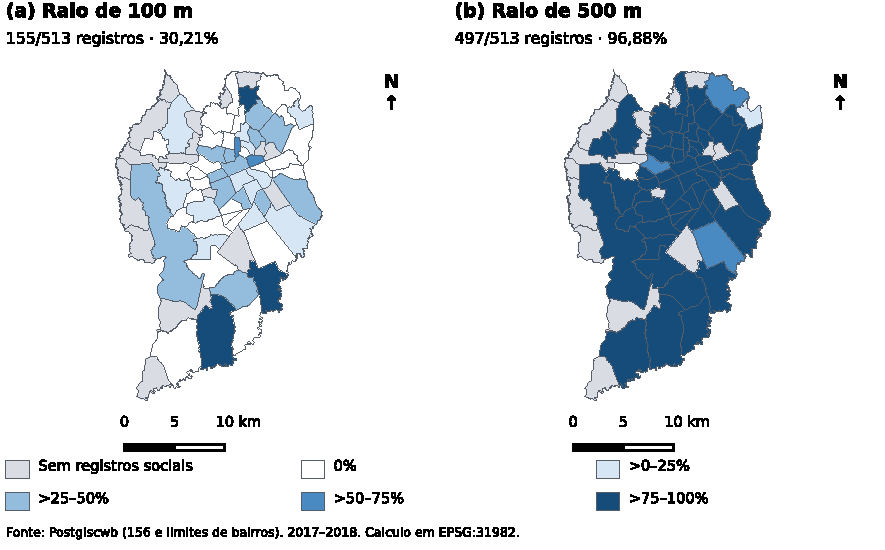
\includegraphics[width=0.78\linewidth]{resultados/mapa_gis.pdf}
\caption{Percentual de registros sociais com pedido de manutenção de iluminação
a até cada raio analisado, por bairro (2017--2018). Cinza: sem registros sociais; branco: 0\%.
Fonte: autores, Postgiscwb; mapas gerados no QGIS.}
\label{fig:mapa}
\end{figure}

\subsection{Limitações e interpretação}
A cobertura de aproximadamente 20\% limita a representatividade, pois não
conhecemos a distribuição dos pedidos sem coordenadas. A associação por endereço
pode gerar erros. Protocolos distintos podem tratar do mesmo local; além disso,
a agregação não exige coincidência de datas e o horário do registro não comprova
ocorrência noturna. As densidades não são taxas populacionais, percentuais com
poucos registros são instáveis, e os pedidos de abordagem social indicam
necessidade de assistência, mas não permitem avaliar o risco de violência.

\section{Conclusão}
O cruzamento espacial mostra concentração de solicitações no Centro e variação
do percentual de proximidade conforme o raio utilizado. Os 96,88\% a 500 m
descrevem proximidade entre pedidos e não permitem inferir risco de violência ou
causalidade.

\begin{thebibliography}{1}
\bibitem{postgis} PostGIS (2026). Documentação: \texttt{ST\_Transform},
\texttt{ST\_Covers}, \texttt{ST\_Area} e \texttt{ST\_DWithin}.
\url{https://postgis.net/docs/}. Acesso em 25 out. 2026.
\end{thebibliography}

\end{document}
